\documentclass[tikz,border=8pt]{standalone}
\usepackage{tikz}
\usetikzlibrary{positioning,arrows.meta}
\begin{document}
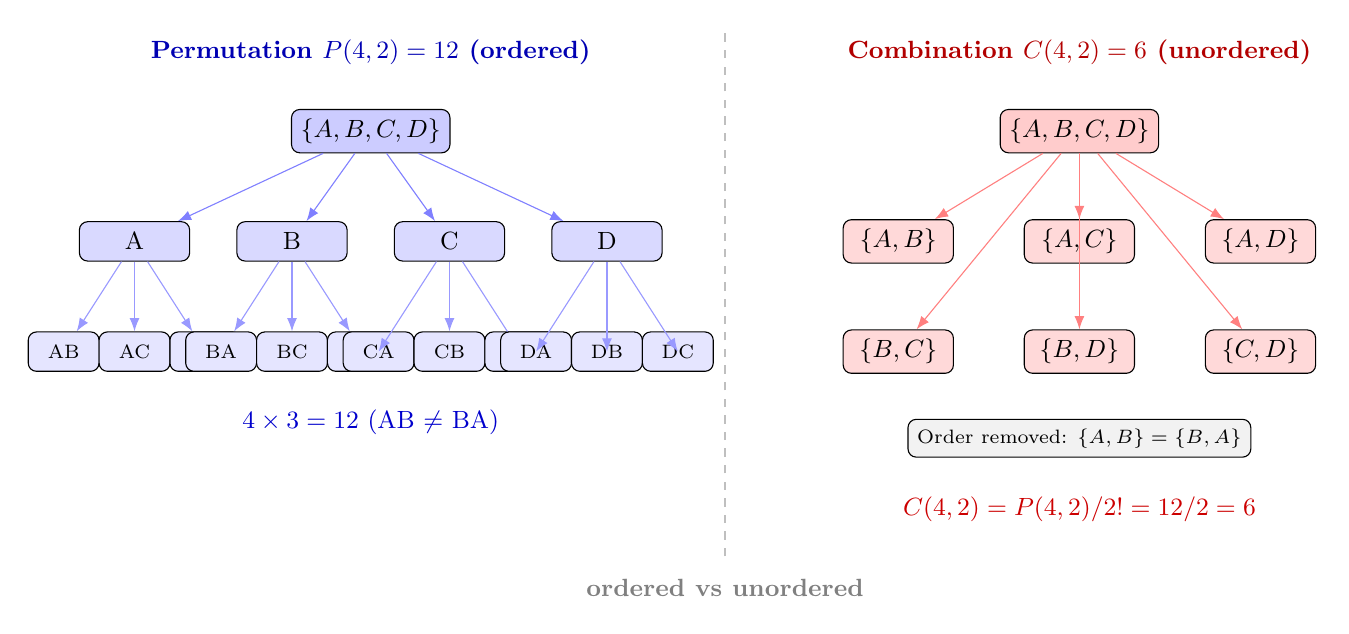
\begin{tikzpicture}[
  nd/.style={draw,rounded corners=3pt,fill=#1,minimum width=1.4cm,
             minimum height=0.5cm,font=\small,align=center},
  >=Latex
]

  %% ===== LEFT: Permutation tree P(4,2)=12 =====
  \node[font=\bfseries\small,blue!70!black] at (-4.5,3.2)
    {Permutation $P(4,2)=12$ (ordered)};

  % Root
  \node[nd=blue!20] (root1) at (-4.5,2.2) {$\{A,B,C,D\}$};

  % Level 1: first element chosen
  \node[nd=blue!15] (La) at (-7.5,0.8) {A};
  \node[nd=blue!15] (Lb) at (-5.5,0.8) {B};
  \node[nd=blue!15] (Lc) at (-3.5,0.8) {C};
  \node[nd=blue!15] (Ld) at (-1.5,0.8) {D};

  \draw[->,thin,blue!50] (root1) -- (La);
  \draw[->,thin,blue!50] (root1) -- (Lb);
  \draw[->,thin,blue!50] (root1) -- (Lc);
  \draw[->,thin,blue!50] (root1) -- (Ld);

  % Level 2: second element (3 options each)
  % From A: B, C, D
  \node[nd=blue!10,minimum width=0.9cm,font=\scriptsize] (AB) at (-8.4,-0.6) {AB};
  \node[nd=blue!10,minimum width=0.9cm,font=\scriptsize] (AC) at (-7.5,-0.6) {AC};
  \node[nd=blue!10,minimum width=0.9cm,font=\scriptsize] (AD) at (-6.6,-0.6) {AD};
  \draw[->,thin,blue!40] (La)--(AB);
  \draw[->,thin,blue!40] (La)--(AC);
  \draw[->,thin,blue!40] (La)--(AD);

  % From B: A, C, D
  \node[nd=blue!10,minimum width=0.9cm,font=\scriptsize] (BA) at (-6.4,-0.6) {};
  \node[nd=blue!10,minimum width=0.9cm,font=\scriptsize] (BC) at (-5.5,-0.6) {};
  \node[nd=blue!10,minimum width=0.9cm,font=\scriptsize] (BD) at (-4.6,-0.6) {};
  \node[font=\scriptsize] at (-6.4,-0.6) {BA};
  \node[font=\scriptsize] at (-5.5,-0.6) {BC};
  \node[font=\scriptsize] at (-4.6,-0.6) {BD};
  \draw[->,thin,blue!40] (Lb)--(BA);
  \draw[->,thin,blue!40] (Lb)--(BC);
  \draw[->,thin,blue!40] (Lb)--(BD);

  % From C: A, B, D
  \node[nd=blue!10,minimum width=0.9cm,font=\scriptsize] at (-4.4,-0.6) {CA};
  \node[nd=blue!10,minimum width=0.9cm,font=\scriptsize] (CBn) at (-3.5,-0.6) {CB};
  \node[nd=blue!10,minimum width=0.9cm,font=\scriptsize] at (-2.6,-0.6) {CD};
  \draw[->,thin,blue!40] (Lc)--(-4.4,-0.6);
  \draw[->,thin,blue!40] (Lc)--(CBn);
  \draw[->,thin,blue!40] (Lc)--(-2.6,-0.6);

  % From D: A, B, C
  \node[nd=blue!10,minimum width=0.9cm,font=\scriptsize] at (-2.4,-0.6) {DA};
  \node[nd=blue!10,minimum width=0.9cm,font=\scriptsize] at (-1.5,-0.6) {DB};
  \node[nd=blue!10,minimum width=0.9cm,font=\scriptsize] at (-0.6,-0.6) {DC};
  \draw[->,thin,blue!40] (Ld)--(-2.4,-0.6);
  \draw[->,thin,blue!40] (Ld)--(-1.5,-0.6);
  \draw[->,thin,blue!40] (Ld)--(-0.6,-0.6);

  \node[font=\small,blue!80!black] at (-4.5,-1.5) {$4\times 3 = 12$ (AB $\neq$ BA)};
  % (permutation count note)

  %% ===== RIGHT: Combination C(4,2)=6 =====
  \node[font=\bfseries\small,red!70!black] at (4.5,3.2)
    {Combination $C(4,2)=6$ (unordered)};

  \node[nd=red!20] (root2) at (4.5,2.2) {$\{A,B,C,D\}$};

  % 6 unique subsets in two rows of 3
  \node[nd=red!15] (R1) at (2.2,0.8) {$\{A,B\}$};
  \node[nd=red!15] (R2) at (4.5,0.8) {$\{A,C\}$};
  \node[nd=red!15] (R3) at (6.8,0.8) {$\{A,D\}$};
  \node[nd=red!15] (R4) at (2.2,-0.6) {$\{B,C\}$};
  \node[nd=red!15] (R5) at (4.5,-0.6) {$\{B,D\}$};
  \node[nd=red!15] (R6) at (6.8,-0.6) {$\{C,D\}$};

  \draw[->,thin,red!50] (root2)--(R1);
  \draw[->,thin,red!50] (root2)--(R2);
  \draw[->,thin,red!50] (root2)--(R3);
  \draw[->,thin,red!50] (root2)--(R4);
  \draw[->,thin,red!50] (root2)--(R5);
  \draw[->,thin,red!50] (root2)--(R6);

  \node[draw,rounded corners=3pt,fill=gray!10,font=\scriptsize,align=center]
    at (4.5,-1.7) {Order removed: $\{A,B\}=\{B,A\}$};
  \node[font=\small,red!80!black] at (4.5,-2.6)
    {$C(4,2) = P(4,2)/2! = 12/2 = 6$};

  %% Divider
  \draw[thick,dashed,gray!50] (0,-3.2) -- (0,3.5);
  \node[font=\bfseries\small,gray,align=center] at (0,-3.6)
    {ordered vs unordered};

\end{tikzpicture}
\end{document}
